\chapter{Návrh}

V této kapitole se budu věnovat návrhu knihovny na automatizaci a jejím funkčním požadavkům.

\section{Účastníci testování}
V rámci knihovny a testovacího běhu se bude vyskytovat několik účastníků testování. Mezi účastníky testování bude patřit:

\begin{description}
    \item[Testovací služba] Služba, která řídí testovací běh.
    \item[Testované zařízení] Hlavní účastník testování, který běží na jiném zařízení, než ze kterého běží testovací služba. 
    \item[Virtuální zařízení] Zařízení, které simuluje nějakou činnost testovaného zařízení. Toto zařízení běží na stejném zařízení, jako testovací služba. 
\end{description}

Testovací služba bude jádrem k řízení testování. Tato služba poběží na samostatném zařízení. Toto zařízení bude běžet na operačním systému Windows. Zařízení bude v rámci infrastruktury serveru Azure DevOps tzv. agent. Agent je výpočetní infrastruktura s nainstalovaným softwarem agenta, který pracuje na jedné určité úloze \cite{agent_docs}. Na agentovi bude server Azure DevOps spouštět testovací běh.

Hlavním cílem je testovat vyvíjený produkt. Toto zařízení v rámci knihovny bude bráno jako testované zařízení. Testovací služba bude podporovat připojení jednoho a více testovaných zařízení. Tato zařízení budou připojeno k zařízení, ze kterého poběží testovací služba, za pomocí Ethernet připojení. 

Součástí knihovny zároveň bude také tzv. virtuální zařízení. Toto zařízení bude primárně sloužit k simulaci nějaké činnosti, kterou by jinak muselo provádět nějaké z testovaných zařízení. Simulováním testovaných zařízení snižujeme hardwarové nároky na testování, což vede ke snížení ekonomických nákladů na testování. Tato zařízení se budou připojovat v závislosti na jednotlivých testech. Následně po skončení testu budou tato zařízení odpojena.

% Testovací knihovna a virtuální participant budou vyvinuti v jazyce \inlinecode{C\#}. Jazyk byl vybrán kvůli dobrému rozsahu již implementovaných komponent a kvůli dobré interoperabilitě se serverem Azure DevOps, díky tomu že obě části jsou vyvíjeny společností Microsoft. Rozhraní pro vyvíjený produkt bude vytvořeno v jazyce \inlinecode{C++}, jelikož tento produkt je v tomto jazyce vyvíjen.

\begin{figure}[htbp]
    \centering 
    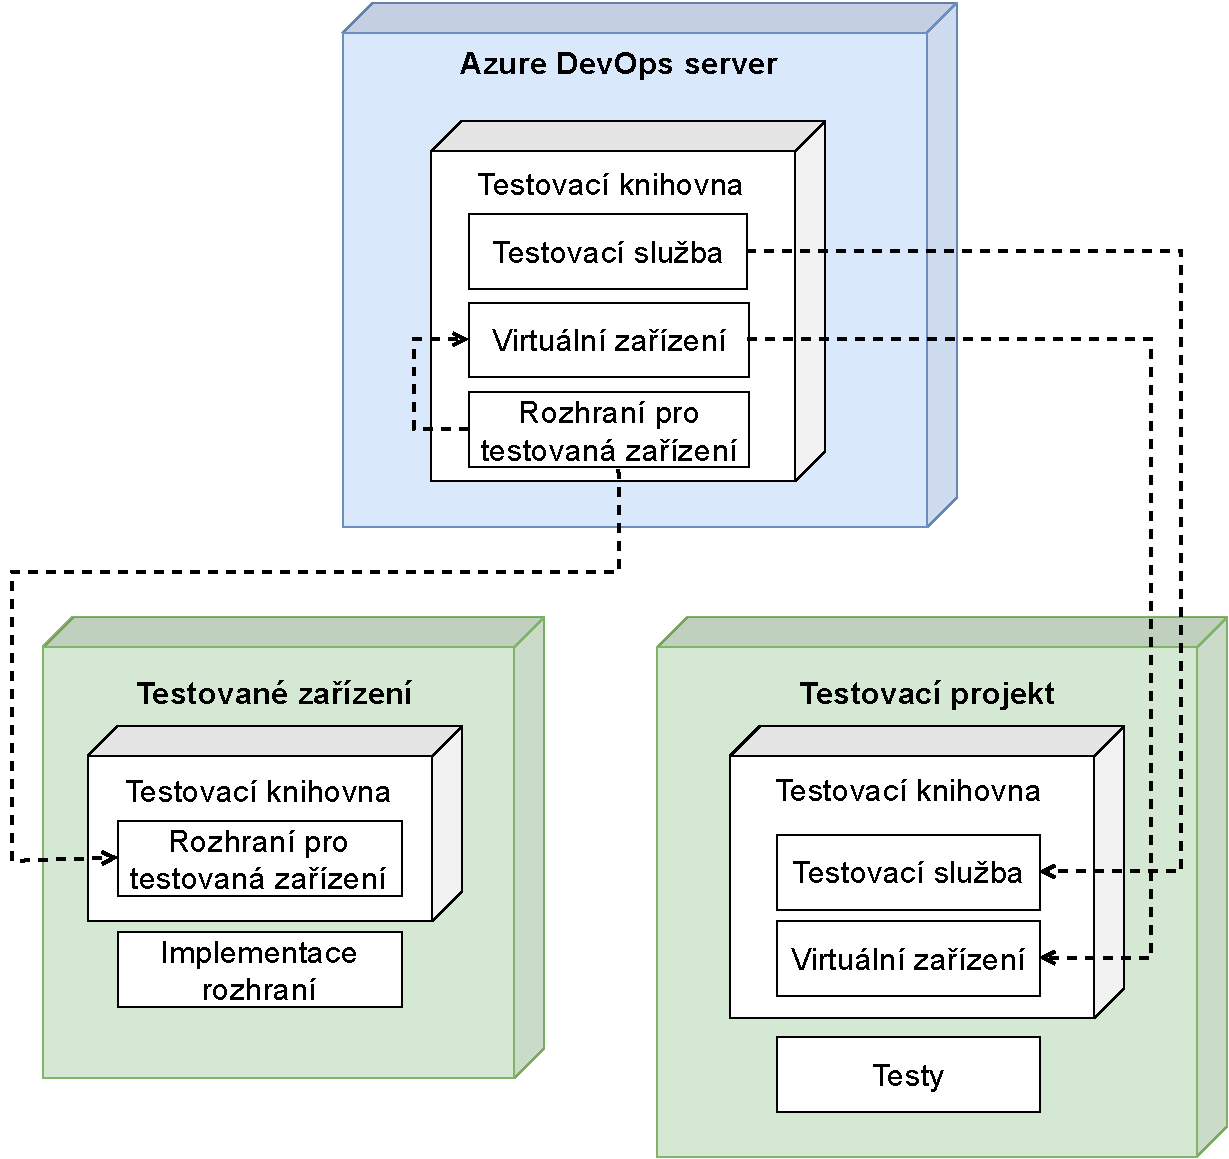
\includegraphics[width=0.95\textwidth]{assets/img/deploymentmodel.pdf}
    \caption{Deployment model}
    \label{fig:deploymodel}
\end{figure}


\section{Komunikace}
Komunikace mezi všemi účastníky testování bude fungovat na principu TCP/IP připojení. Zařízení, na kterém poběží testovací služba, bude sloužit jako server a všichni účastnící testovaní budou klienti, kteří se budou k tomuto zařízení připojovat. 

Jednotlivé zprávy, které budou mezi testovací službou a všemi účastníky testování vyměňovány, budou mít jasně stanovenou strukturu. Složení zprávy lze vidět na obrázku \ref{fig:message}. Jedna zpráva bude obsahovat povinně hlavičku zprávy. Tato hlavička bude obsahovat typ zprávy a délku dat. Data zprávy budou nepovinnou součástí zprávy. 

\begin{figure}[htbp]
    \centering 
    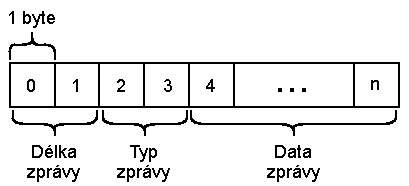
\includegraphics{assets/img/message.pdf}
    \caption{Diagram struktury jedné zprávy}
    \label{fig:message}
\end{figure}

Všechny hodnoty zprávy budou ukládány v kladné (anglicky tzv. unsigned) podobě. Z diagramu zprávy lze vidět, že hlavička zprávy bude o velikosti 4 bajty. Zároveň lze odvodit, že maximální délka dat zprávy bude rovna číslu, které se vejde do dvou bajtů, tedy maximální délka dat zprávy je 65~535 bajtů. Knihovna bude podporovat tyto typy zprávy:

\begin{enumerate}
    \item Zpráva o úspěchu/potvrzení
    \item Zpráva o neúspěchu
    \item Direktiva ke spuštění testu
    \item Direktiva k ukončení testování
\end{enumerate}

Samotná zpráva nebude obsahovat žádné kontrolní data, který by fungovali k detekci možných chyb v komunikaci. Protokol TCP/IP avšak sám obsahuje jednoduchou detekci chyb. V tomto případě bude tato detekce považována jako dostatečná.

Účastníci testování se na začátku připojí k testovací službě a odešlou inicializační zprávu. Tato zpráva bude typu 1 a v datech zprávy bude obsahovat svojí MAC adresu. Výjimkou budou virtuální zařízení, která budou jako svoji MAC adresu odesílat adresu \inlinecode{DE:AD:BE:EF:00:00}. Díky tomu je testovací služba jednoduše identifikuje. Testovací služba následně odešle potvrzovací zprávu o úspěšném připojení s typem 1, bez žádných dat. V případě vzniku chyby služba odešle zprávu typu 2, bez dat. 

Pro započnutí testování a spuštění jednotlivých stádií testování služba odešle všem účastníkům testování zprávu s typem 3. V datech zprávy služba odesílá tyto data:

\begin{enumerate}
    \item Číselnou reprezentaci identifikátoru testu. Ten je uložen v prvních 4 bajtech dat zprávy.
    \item Číselnou reprezentaci identifikátoru, který určuje fázi testu. Uložen je ve dvou bajtech dat zprávy hned za identifikátorem testu. Fáze testování jsou blíže popsány v sekci \ref{test_run}.
\end{enumerate}

Služba následně čeká na odpověď od všech účastníků testování. Účastnící odesílají testovací službě po skončení testovacího stádia zprávu bez dat, s typem 1 v případě úspěchu a s typem 2 v případě neúspěchu. 

Po skončení testování služba odesílá všem účastníkům testování zprávu s typem 4, bez žádných dat. Ukázku komunikace můžeme vidět znázorněnou na sekvenčním diagramu, který je na obrázku \ref{fig:seqdiag}. Na tomto sekvenčním diagramu můžeme vidět výměnu zpráv mezi testovací službou a dvěma účastníky testování během úspěšného testovacího běhu. Direktiva \inlinecode{Message} znázorňuje jednu zprávu, kde v závorkách můžeme vidět nejdříve typ zprávy a následně data zprávy (pokud zpráva nějaká data obsahuje). V diagramu zároveň můžeme vidět cyklus, který reprezentuje spuštění všech testů.

\begin{figure}[htbp]
    \centering 
    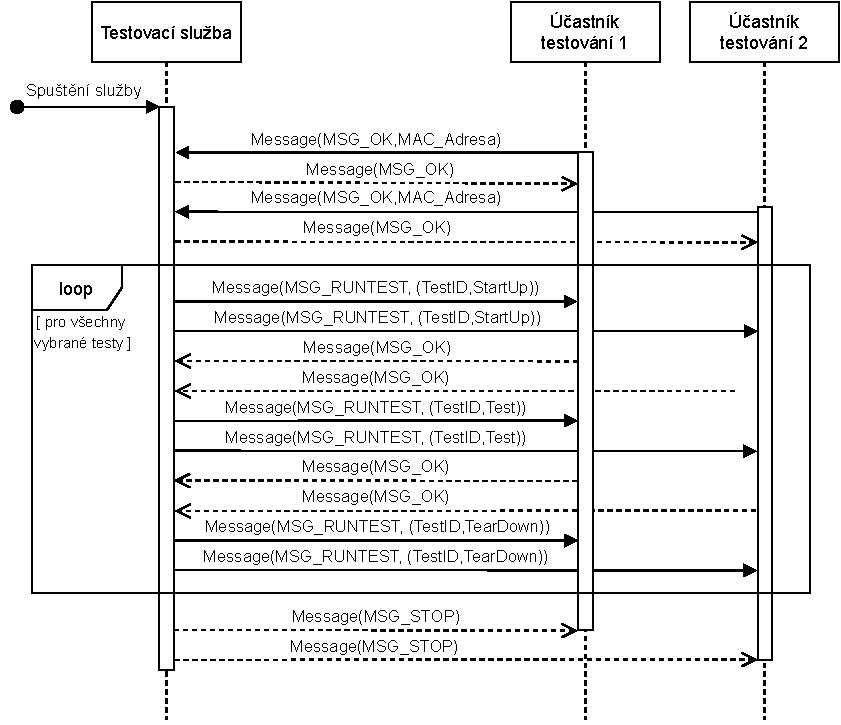
\includegraphics[width=0.95\textwidth]{assets/img/sequencediagram.pdf}
    \caption{Sekvenční diagram znázorňující běh služby}
    \label{fig:seqdiag}
\end{figure}

\section{Testovací služba}
Jak jsem již zmínil, testovací služba bude jádrem celého testování. Tato služba bude řídit celý testovací běh a předávat všem účastníkům testování pokyny. Zároveň bude synchronizovat testovací běh mezi všemi účastníky testování. 

\subsection{Inicializace služby}
Testovací služba započíná běh inicializační fází. Služba v inicializační fázi vytvoří připojení se všemi testovanými zařízeními, dle nadefinované komunikace. Z konfigurace služba bude vědět, kolik testovaných zařízení má očekávat. Inicializační fáze zároveň bude mít definovaný časový limit, který v základu bude 60 sekund, ale bude nastavitelný uživatelem. Testovací služba vyhodnotí inicializační fázi jako úspěšnou, pokud se úspěšně připojí definovaný počet testovaných zařízení. Služba vyhodnocuje neúspěch inicializační fáze v případě že nastanou tyto situace:

\begin{itemize}
    \item vypršení časového limitu na inicializační fázi
    \item chyba v komunikaci, nesprávná komunikace
    \item nepřipojení definovaného počtu zařízení
    \item připojení virtuálního zařízení
\end{itemize}

V případě neúspěchu inicializační fáze služba nastavuje stav služby jako chybný. Testy nebudou provedeny.

\subsection{Spravování virtuálních zařízení}
Jak již bylo nastíněno služba bude podporovat připojení virtuálních zařízení. Toto připojení bude probíhat před započnutím jednotlivých testů. Testovací služba obdrží direktivu k očekávaní připojení virtuálního zařízení. Toto zařízení projde stejnou inicializační fází jako ostatní testovaná zařízení. Služba vyhodnocuje neúspěch připojení virtualizovaného zařízení v těchto případech:

\begin{itemize}
    \item připojení jiného než virtualizovaného zařízení (tedy zařízení ve své zprávě odešle jinou MAC adresu, než je očekávána)
    \item vypršení časového limitu na připojení
    \item chyba v komunikaci
\end{itemize}

V opačném případě služba vyhodnocuje úspěch. Služba následně po testu dokončení testu vysílá všem virtualizovaným zařízením direktivu k ukončení testování a ukončuje spojení s nimi.  

\subsection{Testovací běh}\label{test_run}
Po úspěšné inicializační fázi služba čeká na direktivu ke spuštění testu. Po obdržení této direktivy s identifikátorem testu služba odesílá všem účastníkům testování zprávu k započnutí první fáze testu. Tuto fázi budeme označovat jako přípravu na testování. V této fázi účastníci testovaní připraví všechny potřebné prostředky pro provedení testu. Účastníci následně odesílají zprávu o úspěchu/neúspěchu této fáze. Služba vyhodnocuje fázi jako úspěšnou pokud od všech účastníků obdrží zprávu o úspěchu. V opačném případě vyhodnocuje fázi jako neúspěšnou.

Služba po vyhodnocení úspěchu první fáze přechází do fáze druhé. V této fázi proběhne samotné testování. Služba odešle všem účastníkům zprávu k započnutí této fáze. Následně očekává odpověď od všech účastníků. Služba, stejně jako v přechozí fázi, vyhodnocuje fázi jako úspěšnou, pokud obdrží zprávu o úspěchu od všech účastníků testování. V opačném případě je neúspěšná.

Poslední fází jednotlivého testu je úklid po testu. V této fázi služba opět vyšle zprávu k započnutí fáze. Účastníci testování v této fázi uvádějí zařízení do stavu, ve kterém byl před započnutím testu. Následně zařízení odešlou zprávu o úspěchu/neúspěchu. Vyhodnocení úspěchu/neúspěchu je stejné jako v předchozích fázích.

Testovaná zařízení se v době běhu testu mohou dostat do chybového stavu, ve kterém nebude možné pokračovat testování. Testovací služba bude pro tyto účely předpokládat tyto situace:

\begin{description}
    \item[Neúspěšná fáze] Pro konzistenci testů testovací služba vyžaduje, aby před každým testem a po každém testu testované zařízení bylo ve stejném stavu. Pokud účastník testu odešle neúspěch ve fázi přípravy na test, nebo ve fázi úklidu po testu, tak poté bude tento účastník považován jako chybném stavu. V případě že chyba nastane ve fázi přípravy na test, služba neprovádí fázi testování a přechází do fáze úklidu po testu. 
    \item[Vypršení časového limitu] Testovací služba bude mít definovaný časový limit testu. Tento limit bude definovat dobu, po kterou bude služba po každé fázi testu čekat na odpověď od účastníků testování. V případě vypršení tohoto limitu služba bude předpokládat účastníka opět jako v chybném stavu.
    \item[Chybná komunikace] Stejně jako v inicializační fázi komunikace, která nebude dle definované struktury, vyústí v předpoklad, že testované zařízení je v chybovém stavu. 
\end{description}

Služba vyhodnocuje test jako úspěšný, pokud všechny fáze testu byli úspěšné. Obráceně služba vyhodnocuje test jako neúspěšný pokud jedna z fází byla neúspěšná. V případě nastání chyby, kde testované zařízení je předpokládáno jako v chybovém stavu, testovací služba nastavuje svůj stav jako chybový. Následující testy nebudou provedeny.


\subsection{Ukončení testování}
Testovací služba po obdržení direktivy k ukončení služby odesílá všem účastníkům zprávu k ukončení testovacího běhu. V případě vzniklé chyby testovací služba odesílá tuto direktivu všem zařízením, které považuje jako v nechybovém stavu.


\section{Rozhraní pro testování}
Součástí knihovny taktéž bude rozhraní, pro implementaci zařízení, které bude testováno. Toto rozhraní bude mít jasně definovanou  strukturu, ale zároveň bude co nejjednodušší pro co nejrychlejší implementaci na nově testovaném zařízení. Toto rozhraní bude potom využito pro řízení běhu testu na testovaném zařízení. 

Další součástí bude i rozhraní pro jednotlivé testy. To bude obsahovat jednotlivá stádia testování, která budou mezi všemi zařízeními synchronizovány. Tyto stádia budou, v tom pořadí:
\begin{enumerate}
    \item Příprava na testování -- definování potřebných struktur, inicializace
    \item Testování -- provedení samotného testu
    \item Úklid po testu -- uvolnění využitých zdrojů
\end{enumerate}



% \section{Proces testování}

% Ze předchozí definice testování vyplývá, že knihovna je mířena na automatizaci funkčního testování. Každý testovací běh se bude moct skládat z libovolného počtu registrovaných testů. Na obrázku \ref{fig:act_diag_device} můžeme vidět diagram aktivit testovaného zařízení. Tento diagram ukazuje běh testovaného zařízení. Jeho běh se odvíjí na základě instrukcí, které obdrží od testovací služby. Zařízení nejdříve projde inicializační fázi, ve které se připojí k testovací službě. 


% Samotné kontrolování správnosti testu bude prací jednotlivých testerů. Knihovna pouze dostane informaci o úspěchu nebo neúspěchu jednotlivých synchronizačních částí testovaní, definovaných rozhraním pro testování. Pokud ve fázi přípravy na testování nebo úklidu po testu zařízení vrátí neúspěch, bude toto zařízení považováno jako v chybném stavu. Další testy poté nebudou provedeny. 

% \begin{figure}
%     \centering 
%     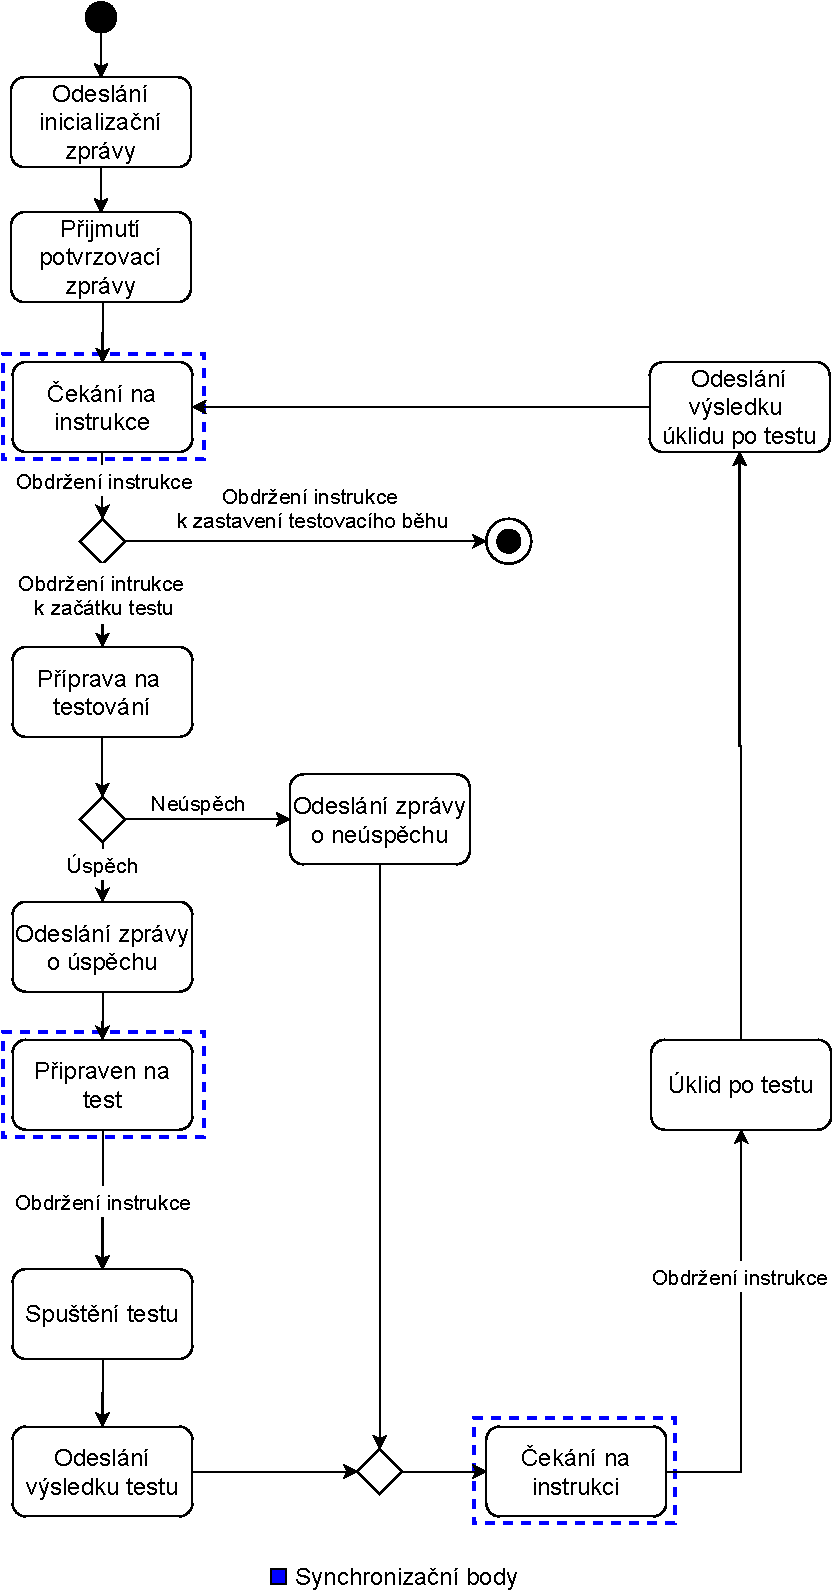
\includegraphics[width=\textwidth]{assets/img/activitydiagramdevice.pdf}
%     \caption{Diagram aktivit testované zařízení}
%     \label{fig:act_diag_device}
% \end{figure}

\section{Propojení se serverem Azure DevOps}
Jedním z cílů této práce je vytvoření takového připojení, aby server Azure DevOps byl schopen spouštět jednotlivé testy. K tomuto propojení využijeme testovací framework MSTest. Vyvíjená testovací knihovna tedy poběží nad tímto testovacím frameworkem. Za pomoci frameworku MSTest bude server Azure DevOps schopen registrovat jednotlivé testy, a spouštět je jednotlivě.

